\documentclass[12pt]{article}
\usepackage[UTF8]{ctex}
\usepackage{amsmath}
\usepackage{amssymb}
\usepackage{amsthm}
\usepackage{esint}
\usepackage{mathrsfs}
\usepackage{graphicx}
\usepackage{enumitem}
\usepackage{geometry}
\usepackage{tocloft}       % 目录美化
\usepackage{fix-cm}       % 消除字体警告
\usepackage{lmodern}      % 消除字体警告
\usepackage{float}        % 图片固定位置
\usepackage{indentfirst}  % 中文首行缩进

% 页面设置
\geometry{a4paper, margin=1in}

% 列表全局样式
\setlist[enumerate]{label=\arabic*., itemsep=1em, topsep=1em, leftmargin=*}
\setlist[enumerate,1]{label=\arabic*.}
\setlist[enumerate,2]{label=(\arabic*)}

% 目录样式（美观、中文适配）
\renewcommand{\cftsecfont}{\bfseries}
\renewcommand{\cftsecleader}{\cftdotfill{\cftdotsep}}

% 超链接（放在最后！）
\usepackage[colorlinks=true, linkcolor=blue, citecolor=blue, urlcolor=blue]{hyperref}

\begin{document}

\begin{titlepage}
    \centering
    \vspace*{2cm}
    
    % 主标题
    {\Huge \bfseries 电磁场作业集 \par}
    \vspace{0.8cm}
    
    % 副标题+课程信息
    {\Large \bfseries 考前复习 \par}
    \vspace{0.4cm}
    {\Large 课程代码：EE2003 \quad 课程名称：电磁场 \par}
    \vspace{0.6cm}
    
    \rule{\linewidth}{0.2mm}
    \vspace{1cm}
    
    % 麦克斯韦名言
    {\itshape \large 电和磁的实验中最明显的现象是，物体之间的相互作用。\par}
    \vspace{0.4cm}
    {\large —— 麦克斯韦 \par}
    \vspace{1.2cm}
    
    % 作者信息
    {\Large 作者：浮萍 \par}
    \vspace{0.3cm}
    {\Large 版本：1.0 \par}
    \vspace{0.3cm}
    {\Large 邮箱：3071974740@qq.com \par}
    \vspace{0.3cm}
    {\Large GitHub：github.com/Duckweed-yhb \par}
    \vspace{1cm}
    
    % 版权信息
    {\large \copyright\ 2026 浮萍 版权所有 \par}
    {\large 未经授权，不得复制、传播或修改 \par}
    \vspace{0.5cm}
    
    \vfill
    {\large 生成日期：\today \par}
\end{titlepage}

\section*{版本说明}
\noindent\textbf{版本：V1.0}
\begin{itemize}
    \item \textbf{配套课程：}课程代码\textbf{EE2003}，课程名称\textbf{电磁场}；
    \item \textbf{参考教材：}《工程电磁场导论》，冯慈璋、马西奎主编，西安交通大学出版社2000版，全书内容严格对标教材目录与期末考点；
    \item \textbf{覆盖范围：}全书五大章节：\textbf{第1章静电场、第2章恒定电场、第3章恒定磁场、第4章时变电磁场、第5章准静态电磁场}，对应教材$\S1\sim\S5$全部课内知识点；
    \item \textbf{内容编排：}
    \begin{itemize}
        \item 1.静电场：电场/电位、高斯定理、边值问题、有限差分法(实验内容)、镜像法、电容、静电能量与力（采用库仑定律+虚位移法求电场力）；
        \item 2.恒定电场：导电媒质电流、局外场强、基本方程、分界面衔接条件、恒定电场与静电场类比、电导；
        \item 3.恒定磁场：磁感应强度、安培环路定律、基本方程、磁矢位、标量磁位、磁场能量与力（洛伦兹公式+虚位移法求磁场力）；
        \item 4.时变电磁场：法拉第电磁感应+全电流定律、麦克斯韦方程组、动态位及其积分解、坡印廷矢量、正弦电磁场、电磁辐射；
        \item 5.准静态场：EQS电准静态/MQS磁准静态场、似稳条件、集肤效应、导体交流内阻抗；
    \end{itemize}
    \item 排版规范：关键公式统一封装\verb|formulaBox|环境，核心定义与考点名词全部\textbf{加粗}标注，各小节以\verb|\hrule|分隔，结构规整便于考前翻阅背诵；
    \item 内容取舍：剔除课外超纲拓展内容，只收录课堂核心考点、典型结论与工程实例，完全贴合课程期末考试大纲；
    \item \textbf{现存缺点：全篇仅文字与公式，无配套几何示意图、原理插图。}
\end{itemize}
\newpage

% 目录
\tableofcontents
\newpage

% 各章节
\section{矢量分析习题解答}

\begin{enumerate}[label=\arabic*.,itemsep=10pt,topsep=5pt,parsep=2pt]

% --------------- 第1题（作业题号4）---------------
\item 设有标量场 $\varphi = 2xy^2 - z^3$，求其在点 $M(2,-1,1)$ 沿 $\overrightarrow{MP}\big(P(3,1,-1)\big)$ 方向的方向导数，以及该点方向导数的最大值。

\textbf{解答：}
\begin{enumerate}[label=(\arabic*),itemsep=5pt,topsep=2pt,parsep=2pt]
\item 求取梯度
\[
\nabla\varphi = \frac{\partial \varphi}{\partial x}\vec{e}_x+\frac{\partial \varphi}{\partial y}\vec{e}_y+\frac{\partial \varphi}{\partial z}\vec{e}_z
= 2y^2\vec{e}_x + 4xy\vec{e}_y - 3z^2\vec{e}_z
\]
将 $M(2,-1,1)$ 代入坐标得：
\[
\nabla\varphi\big|_M = 2\vec{e}_x - 8\vec{e}_y - 3\vec{e}_z
\]

\item 方向矢量 $\overrightarrow{MP}=(1,2,-2)$，其模长
\[
|\overrightarrow{MP}|=\sqrt{1^2+2^2+(-2)^2}=3
\]
单位矢量为
\[
\vec{e}_l = \frac{1}{3}\vec{e}_x + \frac{2}{3}\vec{e}_y - \frac{2}{3}\vec{e}_z
\]

\item 由方向导数公式 $\displaystyle\frac{\partial \varphi}{\partial l}=\nabla\varphi\cdot\vec{e}_l$
\[
\left.\frac{\partial\varphi}{\partial l}\right|_M
=2\cdot\frac13+(-8)\cdot\frac23+(-3)\cdot\left(-\frac23\right)
=-\frac{8}{3}
\]

\item 方向导数最大值出现在梯度同向，大小为梯度模长
\[
\left|\nabla\varphi\big|_M\right|
=\sqrt{2^2+(-8)^2+(-3)^2}
=\sqrt{77}
\]
\end{enumerate}
\textbf{结论：}方向导数$\boxed{-\dfrac{8}{3}}$，最大值$\boxed{\sqrt{77}}$。

% --------------- 第2题（作业题号5）---------------
\item 求标量场 $\varphi = x^3y^4z^2$ 梯度场的散度。

\textbf{解答：}
先求梯度：
\[
\nabla\varphi 
=\frac{\partial\varphi}{\partial x}\vec{e}_x+\frac{\partial\varphi}{\partial y}\vec{e}_y+\frac{\partial\varphi}{\partial z}\vec{e}_z
= 3x^2y^4z^2\vec{e}_x + 4x^3y^3z^2\vec{e}_y + 2x^3y^4z\vec{e}_z
\]
再求梯度的散度（拉普拉斯算子）：
\[
\begin{aligned}
\nabla\cdot(\nabla\varphi)
&=\frac{\partial}{\partial x}(3x^2y^4z^2)+\frac{\partial}{\partial y}(4x^3y^3z^2)+\frac{\partial}{\partial z}(2x^3y^4z) \\
&= 6xy^4z^2 + 12x^3y^2z^2 + 2x^3y^4
\end{aligned}
\]
\textbf{结论：}$\boxed{6xy^4z^2 + 12x^3y^2z^2 + 2x^3y^4}$。

% --------------- 第3题（作业题号7）---------------
\item 设矢量场 $\vec{A} = x^2\vec{e}_x + y^3\vec{e}_y + (3z - x)\vec{e}_z$，求：(1) $M_1(1,0,-1)$ 处散度；(2) $M_2(1,-1,-1)$ 处旋度。

\textbf{解答：}
\begin{enumerate}[label=(\arabic*),itemsep=5pt,topsep=2pt,parsep=2pt]
\item 散度计算
\[
\nabla\cdot\vec{A} 
=\frac{\partial A_x}{\partial x}+\frac{\partial A_y}{\partial y}+\frac{\partial A_z}{\partial z}
=\frac{\partial(x^2)}{\partial x}+\frac{\partial(y^3)}{\partial y}+\frac{\partial(3z-x)}{\partial z}
=2x+3y^2+3
\]
代入 $M_1(1,0,-1)$：
\[
\nabla\cdot\vec{A}\big|_{M_1}=2\times 1+3\times 0^2+3=5
\]

\item 旋度计算
\[
\nabla\times\vec{A} =
\begin{vmatrix}
\vec{e}_x & \vec{e}_y & \vec{e}_z \\
\dfrac{\partial}{\partial x} & \dfrac{\partial}{\partial y} & \dfrac{\partial}{\partial z} \\
x^2 & y^3 & 3z-x
\end{vmatrix}
=\vec{e}_y
\]
该旋度为常矢量，与坐标无关，故 $\nabla\times\vec{A}\big|_{M_2}=\vec{e}_y$。
\end{enumerate}
\textbf{结论：}散度$\boxed{5}$，旋度$\boxed{\vec{e}_y}$。

% --------------- 第4题（作业题号8）---------------
\item 已知电场强度 $\vec{E} = E_0\cos\theta\vec{e}_r - E_0\sin\theta\vec{e}_\theta$，求其散度与旋度。

\textbf{解答：}
在球坐标系中计算散度与旋度，代入化简可得：
\[
\nabla\cdot\vec{E} = 0,\quad \nabla\times\vec{E} = \vec{0}
\]
\textbf{结论：}$\boxed{\nabla\cdot\vec{E}=0,\ \nabla\times\vec{E}=\vec{0}}$。

% --------------- 第5题（作业题号9）---------------
\item 矢量场 $\vec{A}=(x^2-2xy)\vec{e}_x+(y^2-2yz)\vec{e}_y+z(z-2x+1)\vec{e}_z$，求其对半径为$a$、球心在原点的球面外侧的通量。

\textbf{解答：}
由高斯通量定理：
\[
\varPhi=\oiint_S \vec{A}\cdot d\vec{S}=\iiint_V \nabla\cdot\vec{A}\,\mathrm{d}V
\]
计算散度：
\[
\nabla\cdot\vec{A}=1
\]
因此：
\[
\varPhi=\iiint_V 1\,\mathrm{d}V=\frac{4}{3}\pi a^3
\]
\textbf{结论：}通量$\boxed{\dfrac{4}{3}\pi a^3}$。

% --------------- 第6题（作业题号10）---------------
\item 求矢量场 $\vec{A}=xyz(\vec{e}_x+\vec{e}_y+\vec{e}_z)$ 在点 $M(1,3,2)$ 处的旋度，以及绕方向 $\vec{e}_n=\frac{1}{3}(\vec{e}_x+2\vec{e}_y+2\vec{e}_z)$ 的环量面密度。

\textbf{解答：}
旋度计算并代入 $M(1,3,2)$：
\[
\nabla\times\vec{A}\big|_M
=-\vec{e}_x-3\vec{e}_y+4\vec{e}_z
\]
环量面密度为旋度在法向的投影：
\[
\mu_n=(\nabla\times\vec{A})\cdot\vec{e}_n
=\frac{1}{3}
\]
\textbf{结论：}旋度$\boxed{-\vec{e}_x-3\vec{e}_y+4\vec{e}_z}$，环量面密度$\boxed{\dfrac{1}{3}}$。

\end{enumerate}
% 4.静电场习题解答.tex
\section{静电场习题解答}

\begin{enumerate}[label=\arabic*.]
% 第1题
\item 在直角坐标系中，已知电场强度 \(\vec{E} = 6x^2\vec{e}_x + 6y\vec{e}_y + 4\vec{e}_z\ \text{V/m}\)，点 \(M\) 和 \(N\) 的坐标分别为点 \(M(2,6,-1)\)、点 \(N(-3,-3,2)\)，试求：
\begin{enumerate}
    \item \(\varphi_{MN} = ?\)；
    \item 若点 \(Q(4,-2,-35)\) 为参考点，则 \(\varphi_M = ?\)；
    \item 若点 \(P(1,2,-4)\) 处的电位为 2V，则 \(\varphi_N = ?\)
\end{enumerate}

\textbf{解答：}

首先求\textbf{电位函数} \(\varphi(x,y,z)\)。
由 \(\vec{E} = -\nabla\varphi\)，可得：
\[
\begin{cases}
E_x = -\dfrac{\partial \varphi}{\partial x} = 6x^2 \\
E_y = -\dfrac{\partial \varphi}{\partial y} = 6y \\
E_z = -\dfrac{\partial \varphi}{\partial z} = 4
\end{cases}
\]

分别积分得：
\[
\varphi(x,y,z) = -2x^3 - 3y^2 - 4z + C
\]
其中 \(C\) 为积分常数，由\textbf{电位参考点}条件决定。

\vspace{0.5em}
(1) 两点间\textbf{电位差}：
\[
\varphi_{MN} = \varphi_M - \varphi_N
\]

计算 \(\varphi_M\) 和 \(\varphi_N\)：
\[
\varphi_M = -2(2)^3 - 3(6)^2 - 4(-1) + C = -16 - 108 + 4 + C = -120 + C
\]
\[
\varphi_N = -2(-3)^3 - 3(-3)^2 - 4(2) + C = 54 - 27 - 8 + C = 19 + C
\]

因此：
\[
\varphi_{MN} = (-120 + C) - (19 + C) = -139\ \text{V}
\]

\vspace{0.5em}
(2) 以点 \(Q(4,-2,-35)\) 为参考点，即 \(\varphi_Q = 0\)：
\[
\varphi_Q = -2(4)^3 - 3(-2)^2 - 4(-35) + C = -128 - 12 + 140 + C = 0 \implies C=0
\]

电位函数为 \(\varphi(x,y,z) = -2x^3 - 3y^2 - 4z\)。
则 \(M\) 点电位：
\[
\varphi_M = -2(2)^3 - 3(6)^2 - 4(-1) = -16 - 108 + 4 = -120\ \text{V}
\]

\vspace{0.5em}
(3) 已知点 \(P(1,2,-4)\) 处电位为 2V：
\[
\varphi_P = -2(1)^3 - 3(2)^2 - 4(-4) + C = -2 - 12 + 16 + C = 2 + C = 2\ \text{V}
\]

解得 \(C=0\)。
则 \(N\) 点电位：
\[
\varphi_N = -2(-3)^3 - 3(-3)^2 - 4(2) = 54 - 27 - 8 = 19\ \text{V}
\]

\vspace{1em}

% 第2题
\item 在直角坐标系中电荷分布为 \(\rho(x,y,z)\)，试求电场强度 \(\vec{E}\)，其中
\[
\rho(x,y,z) =
\begin{cases}
\rho_0, & x = 0 \\
0, & x \neq 0
\end{cases}
\]

\textbf{解答：}

题目中电荷仅分布在 \(x=0\) 平面上，属于\textbf{面电荷分布}，其\textbf{面电荷密度}为：
\[
\rho_s = \rho_0 \quad (\text{单位：C/m}^2)
\]

根据对称性，电场强度 \(\vec{E}\) 只有 \(x\) 方向分量，且与 \(y,z\) 无关。利用\textbf{高斯定理}求解：

取高斯面为跨接在 \(x=0\) 平面两侧的柱形闭合面，柱体轴线沿 \(x\) 轴，端面垂直于 \(x\) 轴，面积为 \(A\)。

由高斯定理：
\[
\oint_S \vec{E} \cdot d\vec{S} = \frac{Q_{\text{enc}}}{\varepsilon_0}
\]
其中闭合面内包围电荷 \(Q_{\text{enc}} = \rho_s A = \rho_0 A\)。

\begin{itemize}
    \item 对于 \(x>0\) 区域：电场方向沿 \(+\vec{e}_x\)，\(E_x = E\)
    \item 对于 \(x<0\) 区域：电场方向沿 \(-\vec{e}_x\)，\(E_x = -E\)
\end{itemize}

高斯面通量仅由两个端面贡献：
\[
\oint_S \vec{E} \cdot d\vec{S} = E \cdot A + E \cdot A = 2EA
\]

代入高斯定理：
\[
2EA = \frac{\rho_0 A}{\varepsilon_0} \implies E = \frac{\rho_0}{2\varepsilon_0}
\]

因此，电场强度为：
\[
\vec{E}(x) =
\begin{cases}
\dfrac{\rho_0}{2\varepsilon_0} \vec{e}_x, & x > 0 \\
-\dfrac{\rho_0}{2\varepsilon_0} \vec{e}_x, & x < 0
\end{cases}
\]

\vspace{1em}

% 第3题
\item 对于下面给出的几种 \(\vec{D}\) 场，试求相应的\textbf{体电荷密度}表达式：
\begin{enumerate}
    \item \(\displaystyle \vec{D} = \frac{4xy}{z}\vec{e}_x + \frac{2x^2}{z}\vec{e}_y - \frac{2x^2y}{z^2}\vec{e}_z\)；
    \item \(\displaystyle \vec{D} = z\sin\phi\vec{e}_\rho + z\cos\phi\vec{e}_\phi + \rho\sin\phi\vec{e}_z\)
\end{enumerate}

\textbf{解答：}

根据介质中高斯定理微分形式，自由体电荷密度 \(\rho_f = \nabla \cdot \vec{D}\)。

\vspace{0.5em}
(1) 直角坐标系下的\textbf{散度}：
\[
\nabla \cdot \vec{D} = \frac{\partial D_x}{\partial x} + \frac{\partial D_y}{\partial y} + \frac{\partial D_z}{\partial z}
\]

分别求偏导：
\[
\frac{\partial D_x}{\partial x} = \frac{\partial}{\partial x}\left( \frac{4xy}{z} \right) = \frac{4y}{z}
\]
\[
\frac{\partial D_y}{\partial y} = \frac{\partial}{\partial y}\left( \frac{2x^2}{z} \right) = 0
\]
\[
\frac{\partial D_z}{\partial z} = \frac{\partial}{\partial z}\left( -\frac{2x^2y}{z^2} \right) = \frac{4x^2y}{z^3}
\]

因此：
\[
\rho_f = \frac{4y}{z} + \frac{4x^2y}{z^3} = \frac{4y}{z}\left( 1 + \frac{x^2}{z^2} \right)
\]

\vspace{0.5em}
(2) 柱坐标系下的散度：
\[
\nabla \cdot \vec{D} = \frac{1}{\rho}\frac{\partial (\rho D_\rho)}{\partial \rho} + \frac{1}{\rho}\frac{\partial D_\phi}{\partial \phi} + \frac{\partial D_z}{\partial z}
\]

分别求偏导：
\[
\frac{1}{\rho}\frac{\partial (\rho D_\rho)}{\partial \rho} = \frac{1}{\rho}\frac{\partial}{\partial \rho}\left( \rho \cdot z\sin\phi \right) = \frac{z\sin\phi}{\rho}
\]
\[
\frac{1}{\rho}\frac{\partial D_\phi}{\partial \phi} = \frac{1}{\rho}\frac{\partial}{\partial \phi}\left( z\cos\phi \right) = -\frac{z\sin\phi}{\rho}
\]
\[
\frac{\partial D_z}{\partial z} = \frac{\partial}{\partial z}\left( \rho\sin\phi \right) = 0
\]

因此：
\[
\rho_f = \frac{z\sin\phi}{\rho} - \frac{z\sin\phi}{\rho} + 0 = 0
\]

\vspace{1em}

% 第4题
\item 在空间区域为 \(x=0\) 到 \(1\)，\(y=0\) 到 \(2\)，\(z=0\) 到 \(3\) 的平行六面体内，有矢量场 \(\vec{D} = 2xy\vec{e}_x + x^2\vec{e}_y\ \text{C/m}^2\)。试计算平行六面体内的\textbf{总电荷量}。

\textbf{解答：}

根据高斯定理，闭合曲面内的总电荷量等于电位移矢量的体积分：
\[
Q = \iiint_V \rho_f \, dV = \iiint_V (\nabla \cdot \vec{D}) \, dV
\]

首先计算体电荷密度 \(\rho_f = \nabla \cdot \vec{D}\)：
\[
\nabla \cdot \vec{D} = \frac{\partial D_x}{\partial x} + \frac{\partial D_y}{\partial y} + \frac{\partial D_z}{\partial z}
\]

其中：
\[
D_x = 2xy, \quad D_y = x^2, \quad D_z = 0
\]

因此：
\[
\frac{\partial D_x}{\partial x} = 2y, \quad \frac{\partial D_y}{\partial y} = 0, \quad \frac{\partial D_z}{\partial z} = 0
\]

所以：
\[
\rho_f = 2y
\]

对 \(\rho_f\) 在平行六面体内积分，求总电荷量：
\[
Q = \int_{x=0}^{1} \int_{y=0}^{2} \int_{z=0}^{3} 2y \, dz \, dy \, dx
\]

分步计算：
\begin{enumerate}
    \item 对 \(z\) 积分：
    \[
    \int_{z=0}^{3} dz = 3
    \]
    \item 对 \(y\) 积分：
    \[
    \int_{y=0}^{2} 2y \cdot 3 \, dy = 3 \int_{0}^{2} 2y \, dy = 3 \left[ y^2 \right]_0^2 = 12
    \]
    \item 对 \(x\) 积分：
    \[
    Q = \int_{x=0}^{1} 12 \, dx = 12
    \]
\end{enumerate}

因此，平行六面体内的总电荷量为 \(Q = 12\ \text{C}\)。

\vspace{1em}

% 第5题
\item 无限长同轴圆柱面，半径分别为 \(a\) 和 \(b\)（\(b > a\)），每单位长度上电荷：内柱上为 \(\tau\)，外柱为 \(-\tau\)。求真空中带电面之间的\textbf{电压}。

\textbf{解答：}

根据电荷分布的轴对称性，两圆柱面之间（\(a < \rho < b\)）的电场强度可由高斯定理求得。

取半径为 \(\rho\)、长度为 \(l\) 的同轴圆柱面为高斯面，由高斯定理：
\[
\oint_S \vec{E} \cdot d\vec{S} = \frac{Q_{\text{enc}}}{\varepsilon_0}
\]

高斯面内包围的电荷为 \(Q_{\text{enc}} = \tau l\)，电场仅沿径向 \(\vec{e}_\rho\) 方向，因此：
\[
E \cdot 2\pi\rho l = \frac{\tau l}{\varepsilon_0}
\]

解得：
\[
E(\rho) = \frac{\tau}{2\pi\varepsilon_0 \rho} \quad (a < \rho < b)
\]

两圆柱面之间的电压（电位差）为：
\[
U_{ab} = \varphi_a - \varphi_b = \int_{a}^{b} \vec{E} \cdot d\vec{\rho}
\]

代入电场表达式：
\[
U_{ab} = \int_{a}^{b} \frac{\tau}{2\pi\varepsilon_0 \rho} d\rho = \frac{\tau}{2\pi\varepsilon_0} \ln \frac{b}{a}
\]

因此，两圆柱面之间的电压为：
\[
U = \frac{\tau}{2\pi\varepsilon_0} \ln \frac{b}{a}
\]

\vspace{1em}

% 第6题
\item 从静电场基本性质出发，证明当电介质均匀时，\textbf{极化电荷密度} \(\rho_p\) 存在的条件是自由电荷的体密度 \(\rho\) 不为零，且有关系式
\[
\rho_p = -\left(1 - \frac{\varepsilon_0}{\varepsilon}\right)\rho
\]

\textbf{证明：}

1. 根据介质中的高斯定理微分形式：
\[
\nabla \cdot \vec{D} = \rho
\]
其中电位移矢量 \(\vec{D} = \varepsilon \vec{E}\)（均匀线性介质），代入得：
\[
\nabla \cdot (\varepsilon \vec{E}) = \rho
\]

由于介质均匀，\(\varepsilon\) 为常数，可提出散度外：
\[
\varepsilon \nabla \cdot \vec{E} = \rho \implies \nabla \cdot \vec{E} = \frac{\rho}{\varepsilon}
\]

\vspace{0.5em}
2. 同时，电场强度的散度满足：
\[
\nabla \cdot \vec{E} = \frac{\rho + \rho_p}{\varepsilon_0}
\]
其中 \(\rho_p\) 为极化电荷体密度。

\vspace{0.5em}
3. 联立上述两式：
\[
\frac{\rho}{\varepsilon} = \frac{\rho + \rho_p}{\varepsilon_0}
\]

交叉相乘并整理：
\[
\rho \varepsilon_0 = \varepsilon(\rho + \rho_p)
\]
\[
\varepsilon \rho_p = \rho \varepsilon_0 - \varepsilon \rho
\]
\[
\rho_p = \rho \left( \frac{\varepsilon_0}{\varepsilon} - 1 \right) = -\left(1 - \frac{\varepsilon_0}{\varepsilon}\right)\rho
\]

\vspace{0.5em}
4. 结论：
\begin{itemize}
    \item 若 \(\rho = 0\)，则 \(\rho_p = 0\)，即均匀介质内部无自由电荷时，也无极化体电荷；
    \item 只有当 \(\rho \neq 0\) 时，\(\rho_p\) 才不为零，且满足 \(\rho_p = -\left(1 - \frac{\varepsilon_0}{\varepsilon}\right)\rho\)。
\end{itemize}

\vspace{1em}

% 第7题
\item 已知真空中有三个点电荷 \(q_1 = 1\,\text{C}\)，\(q_2 = 1\,\text{C}\)，\(q_3 = 4\,\text{C}\)，分别位于 \((1,0,0)\)、\((0,1,0)\)、\((-1,0,0)\) 点，求 \((1,1,1)\) 点的\textbf{电场强度}。

\textbf{解答：}

点电荷的电场强度公式为：
\[
\vec{E} = \frac{1}{4\pi\varepsilon_0} \frac{q}{|\vec{r} - \vec{r}'|^3} (\vec{r} - \vec{r}')
\]
其中 \(\vec{r}=(1,1,1)\) 为场点，\(\vec{r}'\) 为源点。

\vspace{0.5em}
1. 计算 \(q_1\) 在 \((1,1,1)\) 点的电场 \(\vec{E}_1\)
\[
\vec{r} - \vec{r}_1' = (0,1,1),\quad |\vec{r} - \vec{r}_1'| = \sqrt{2}
\]
\[
\vec{E}_1 = \frac{1}{4\pi\varepsilon_0} \frac{1}{2\sqrt{2}} (0,1,1)
\]

\vspace{0.5em}
2. 计算 \(q_2\) 在 \((1,1,1)\) 点的电场 \(\vec{E}_2\)
\[
\vec{r} - \vec{r}_2' = (1,0,1),\quad |\vec{r} - \vec{r}_2'| = \sqrt{2}
\]
\[
\vec{E}_2 = \frac{1}{4\pi\varepsilon_0} \frac{1}{2\sqrt{2}} (1,0,1)
\]

\vspace{0.5em}
3. 计算 \(q_3\) 在 \((1,1,1)\) 点的电场 \(\vec{E}_3\)
\[
\vec{r} - \vec{r}_3' = (2,1,1),\quad |\vec{r} - \vec{r}_3'| = \sqrt{6}
\]
\[
\vec{E}_3 = \frac{1}{4\pi\varepsilon_0} \frac{4}{6\sqrt{6}} (2,1,1) = \frac{1}{4\pi\varepsilon_0} \frac{2}{3\sqrt{6}} (2,1,1)
\]

\vspace{0.5em}
4. 总电场强度叠加 \(\vec{E} = \vec{E}_1 + \vec{E}_2 + \vec{E}_3\)
\[
E_x = \frac{1}{4\pi\varepsilon_0} \left( 0 + \frac{1}{2\sqrt{2}} + \frac{4}{3\sqrt{6}} \right)
\]
\[
E_y = \frac{1}{4\pi\varepsilon_0} \left( \frac{1}{2\sqrt{2}} + 0 + \frac{2}{3\sqrt{6}} \right)
\]
\[
E_z = \frac{1}{4\pi\varepsilon_0} \left( \frac{1}{\sqrt{2}} + \frac{2}{3\sqrt{6}} \right)
\]

整理可得：
\[
\vec{E} = \frac{1}{4\pi\varepsilon_0} \left[
\left( \frac{1}{2\sqrt{2}} + \frac{4}{3\sqrt{6}} \right)\vec{e}_x
+ \left( \frac{1}{2\sqrt{2}} + \frac{2}{3\sqrt{6}} \right)\vec{e}_y
+ \left( \frac{1}{\sqrt{2}} + \frac{2}{3\sqrt{6}} \right)\vec{e}_z
\right] \quad (\text{V/m})
\]

\vspace{1em}

% 第8题
\item 有一分区均匀理想电介质电场，区域1（\(z<0\)）中的相对介电常数为 \(\varepsilon_{r1}\)，区域2（\(z>0\)）中的相对介电常数为 \(\varepsilon_{r2}\)。已知 \(\vec{E}_1 = 20\vec{e}_x - 10\vec{e}_y + 50\vec{e}_z\)，求 \(\vec{D}_1\)、\(\vec{E}_2\) 和 \(\vec{D}_2\)。

\textbf{解答：}

设分界面为 \(z=0\) 平面，法向单位矢量 \(\vec{e}_n = \vec{e}_z\)，且分界面上无自由面电荷（\(\sigma_f=0\)）。

\vspace{0.5em}
1. 求区域1的电位移矢量 \(\vec{D}_1\)
\[
\vec{D}_1 = \varepsilon_1 \vec{E}_1 = \varepsilon_{r1}\varepsilon_0 \vec{E}_1
\]
代入 \(\vec{E}_1\)：
\[
\vec{D}_1 = \varepsilon_{r1}\varepsilon_0 (20\vec{e}_x - 10\vec{e}_y + 50\vec{e}_z)
\]

\vspace{0.5em}
2. 利用\textbf{分界面衔接条件}求 \(\vec{E}_2\)
\begin{itemize}
    \item 切向分量连续：\(\vec{E}_{2t} = \vec{E}_{1t} = 20\vec{e}_x - 10\vec{e}_y\)
    \item 法向分量连续：\(D_{2n} = D_{1n} = 50\varepsilon_{r1}\varepsilon_0\)
\end{itemize}

由 \(\vec{D}_2 = \varepsilon_{r2}\varepsilon_0 \vec{E}_2\)，得：
\[
E_{2n} = \frac{50\varepsilon_{r1}}{\varepsilon_{r2}}
\]

故：
\[
\vec{E}_2 = 20\vec{e}_x - 10\vec{e}_y + \frac{50\varepsilon_{r1}}{\varepsilon_{r2}} \vec{e}_z
\]

\vspace{0.5em}
3. 求区域2的电位移矢量 \(\vec{D}_2\)
\[
\vec{D}_2 = \varepsilon_{r2}\varepsilon_0 \vec{E}_2
= \varepsilon_{r2}\varepsilon_0 (20\vec{e}_x - 10\vec{e}_y) + 50\varepsilon_{r1}\varepsilon_0 \vec{e}_z
\]

最终结果：
\[
\vec{D}_1 = \varepsilon_{r1}\varepsilon_0 \left(20\vec{e}_x - 10\vec{e}_y + 50\vec{e}_z\right)
\]
\[
\vec{E}_2 = 20\vec{e}_x - 10\vec{e}_y + \frac{50\varepsilon_{r1}}{\varepsilon_{r2}} \vec{e}_z
\]
\[
\vec{D}_2 = \varepsilon_{r2}\varepsilon_0 (20\vec{e}_x - 10\vec{e}_y) + 50\varepsilon_{r1}\varepsilon_0 \vec{e}_z
\]

\vspace{1em}

% 第9题
\item 在平行平面静电场中，边界线的某一部分与一条电场强度线重合。这部分边界线的边界条件如何表示？

\textbf{解答：}

平行平面静电场中，电位函数为 \(\varphi(x,y)\)，电场强度与电位的关系为 \(\vec{E} = -\nabla\varphi\)，电场线的切线方向与 \(\vec{E}\) 方向一致。

由于该部分边界线与电场线重合，因此电场强度在边界的法向分量为零：
\[
E_n = 0
\]

又因为 \(E_n = -\dfrac{\partial \varphi}{\partial n}\)，因此电位的法向导数为零：
\[
\dfrac{\partial \varphi}{\partial n} = 0
\]

这是该部分边界条件，属于\textbf{齐次诺伊曼边界条件}，表示边界线是一条等通量线（或电力线），没有电位移矢量穿过该边界。

\vspace{1em}

% 第10题
\item 面积为 \(A\)，间距为 \(d\) 的平板电容器电压为 \(U\)，介电常数为 \(\varepsilon\)，厚度为 \(t\) 的介质板分别如图(a)、(b)所示的方式放置在导电平板之间。分别计算两种情况下电容器中电场及电荷的分布。

\begin{center}
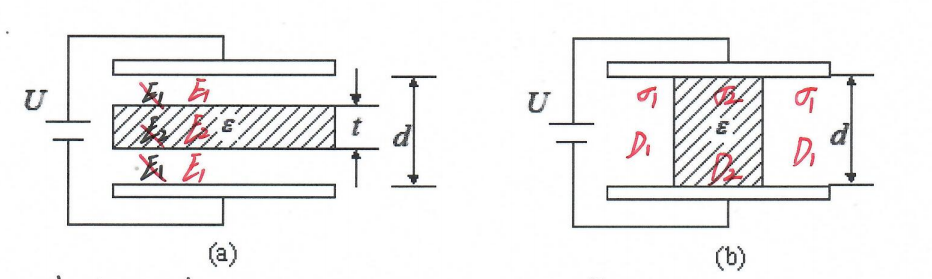
\includegraphics[width=0.8\textwidth]{4.10.png}
\end{center}

\textbf{解答：}

\textbf{(a) 介质板沿电场方向插入（串联模型）}

1. \textbf{电场强度}

介质板厚度为 \(t\)，剩余空气层厚度为 \(d-t\)，两部分电场分别为 \(E_1\)（空气）和 \(E_2\)（介质）。

由电压关系：
\[
U = E_1(d-t) + E_2 t
\]

分界面上电位移法向分量连续（无自由电荷）：
\[
D_1 = D_2 \implies \varepsilon_0 E_1 = \varepsilon E_2
\]

联立解得：
\[
E_1 = \frac{\varepsilon U}{\varepsilon_0 t + \varepsilon(d-t)}, \quad
E_2 = \frac{\varepsilon_0 U}{\varepsilon_0 t + \varepsilon(d-t)}
\]

\vspace{0.5em}
2. \textbf{电荷分布}

极板上的自由电荷面密度由电位移决定：
\[
\sigma = D_1 = \varepsilon_0 E_1 = \frac{\varepsilon_0 \varepsilon U}{\varepsilon_0 t + \varepsilon(d-t)}
\]

介质表面的极化电荷面密度为：
\[
\sigma_p = P = (\varepsilon - \varepsilon_0)E_2 = \frac{(\varepsilon - \varepsilon_0)\varepsilon_0 U}{\varepsilon_0 t + \varepsilon(d-t)}
\]

\vspace{1em}
\textbf{(b) 介质板垂直电场方向插入（并联模型）}

1. \textbf{电场强度}

介质板与空气层并排，极板间距均为 \(d\)，电压均为 \(U\)，因此：
\[
E_1 = E_2 = \frac{U}{d}
\]

\vspace{0.5em}
2. \textbf{电荷分布}

空气部分电位移：
\[
D_1 = \varepsilon_0 E_1 = \frac{\varepsilon_0 U}{d}
\]

介质部分电位移：
\[
D_2 = \varepsilon E_2 = \frac{\varepsilon U}{d}
\]

对应极板上的自由电荷面密度分别为：
\[
\sigma_1 = D_1 = \frac{\varepsilon_0 U}{d}, \quad
\sigma_2 = D_2 = \frac{\varepsilon U}{d}
\]

介质表面的极化电荷面密度为：
\[
\sigma_p = P = (\varepsilon - \varepsilon_0)E_2 = \frac{(\varepsilon - \varepsilon_0)U}{d}
\]

\vspace{1em}

% 第11题
\item 写出下列静电场的边值问题：

\begin{center}
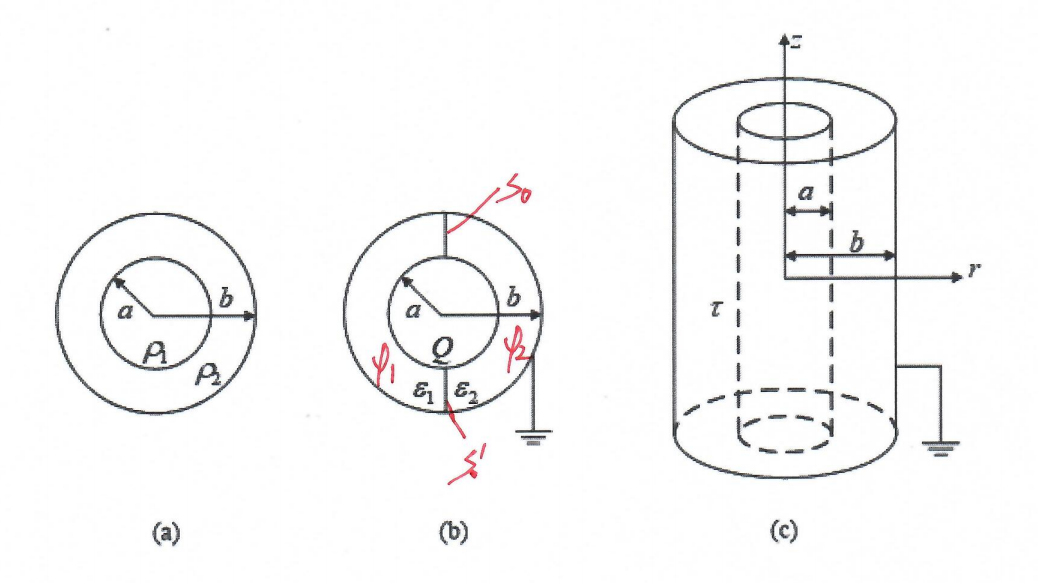
\includegraphics[width=0.8\textwidth]{4.11.png}
\end{center}

\begin{enumerate}
    \item 电荷体密度分别为 \(\rho_1\) 和 \(\rho_2\)，半径分别为 \(a\) 与 \(b\) 的双层同心带电球体，如图(a)所示；
    \item 在两同心导体球壳间，左半部和右半部分别填充介电常数为 \(\varepsilon_1\) 与 \(\varepsilon_2\) 的均匀介质，内球壳带总电荷量为 \(Q\)，外球壳接地，如图(b)所示；
    \item 半径分别为 \(a\) 与 \(b\) 的无限长空心同轴圆柱面导体，内圆柱表面上单位长度的电量为 \(\tau\)，外圆柱面导体接地，如图(c)所示。
\end{enumerate}

\textbf{解答：}

\vspace{0.5em}
(1) 双层同心带电球体（图a）

设电位分布为 \(\varphi(r)\)，根据球对称性，电位仅与径向坐标 \(r\) 有关，分区域写出方程与边界条件：

- 区域1：\(0 \le r < a\)
  \[
  \nabla^2 \varphi_1 = -\frac{\rho_1}{\varepsilon_0}
  \]
- 区域2：\(a < r < b\)
  \[
  \nabla^2 \varphi_2 = -\frac{\rho_2}{\varepsilon_0}
  \]
- 区域3：\(r > b\)
  \[
  \nabla^2 \varphi_3 = 0
  \]

边界条件：
\begin{align*}
& r=0: & & \varphi_1 \text{ 有限} \\
& r=a: & & \varphi_1 = \varphi_2,\quad \varepsilon_0 \frac{d\varphi_1}{dr} = \varepsilon_0 \frac{d\varphi_2}{dr} \\
& r=b: & & \varphi_2 = \varphi_3,\quad \varepsilon_0 \frac{d\varphi_2}{dr} = \varepsilon_0 \frac{d\varphi_3}{dr} \\
& r\to\infty: & & \varphi_3 \to 0
\end{align*}

\vspace{0.5em}
(2) 分区介质同心导体球壳（图b）

设左半区域（\(\varepsilon_1\)）电位为 \(\varphi_1(r)\)，右半区域（\(\varepsilon_2\)）电位为 \(\varphi_2(r)\)，根据球对称性，电位仅与 \(r\) 有关，且两区域电位相等 \(\varphi_1(r)=\varphi_2(r)=\varphi(r)\)。

控制方程（\(a<r<b\)）：
\[
\nabla^2 \varphi = 0
\]

边界条件：
\begin{align*}
& r=a: & & -\left( \varepsilon_1 \int_{\text{左半球}} \frac{\partial \varphi}{\partial r} dS + \varepsilon_2 \int_{\text{右半球}} \frac{\partial \varphi}{\partial r} dS \right) = Q \\
& r=b: & & \varphi = 0 \\
& \theta=\pi/2: & & \varphi_1 = \varphi_2,\quad \varepsilon_1 \frac{\partial \varphi_1}{\partial \theta} = \varepsilon_2 \frac{\partial \varphi_2}{\partial \theta}
\end{align*}

\vspace{0.5em}
(3) 无限长同轴圆柱导体（图c）

设电位分布为 \(\varphi(\rho)\)，根据轴对称性，电位仅与径向坐标 \(\rho\) 有关，区域 \(a<\rho<b\) 内：

控制方程：
\[
\nabla^2 \varphi = 0
\]

边界条件：
\begin{align*}
& \rho=a: & & -2\pi a \varepsilon_0 \frac{d\varphi}{d\rho}\bigg|_{\rho=a} = \tau \\
& \rho=b: & & \varphi = 0
\end{align*}

\vspace{1em}

% 第12题
\item 两个小球半径分别为 \(a=1\,\text{cm}\)，相距为 \(d=20\,\text{cm}\)，位于空气中。
\begin{enumerate}
    \item 若已知 \(\varphi_1\)，\(\varphi_2\)，求 \(q_1\) 和 \(q_2\)；
    \item 若已知 \(\varphi_1\)，\(q_2\)，求 \(q_1\) 和 \(\varphi_2\)；
    \item 问用什么办法使小球1带电荷 \(q_1 = 10^{-8}\,\text{C}\)，小球2不带电荷。
\end{enumerate}

\textbf{解答：}

由于 \(d=20\,\text{cm} \gg a=1\,\text{cm}\)，可近似认为每个小球上的电荷分布均匀，即把它们看作点电荷。设两球电位分别为 \(\varphi_1\) 和 \(\varphi_2\)，由电位叠加原理：
\[
\begin{cases}
\varphi_1 = \frac{1}{4\pi\varepsilon_0} \left( \frac{q_1}{a} + \frac{q_2}{d} \right) \\
\varphi_2 = \frac{1}{4\pi\varepsilon_0} \left( \frac{q_1}{d} + \frac{q_2}{a} \right)
\end{cases}
\]

\vspace{0.5em}
(1) 已知 \(\varphi_1, \varphi_2\)，求 \(q_1, q_2\)。

联立上述方程组，解得：
\[
q_1 = \frac{4\pi\varepsilon_0}{1 - (a/d)^2} \left( a\varphi_1 - \frac{a^2}{d}\varphi_2 \right)
\]
\[
q_2 = \frac{4\pi\varepsilon_0}{1 - (a/d)^2} \left( a\varphi_2 - \frac{a^2}{d}\varphi_1 \right)
\]

\vspace{0.5em}
(2) 已知 \(\varphi_1, q_2\)，求 \(q_1, \varphi_2\)。

由第一个方程解得 \(q_1\)：
\[
q_1 = 4\pi\varepsilon_0 a\varphi_1 - \frac{a}{d}q_2
\]
将 \(q_1\) 代入第二个方程，得 \(\varphi_2\)：
\[
\varphi_2 = \frac{1}{4\pi\varepsilon_0} \left( \frac{4\pi\varepsilon_0 a\varphi_1 - \frac{a}{d}q_2}{d} + \frac{q_2}{a} \right) = \frac{a}{d}\varphi_1 + \frac{q_2}{4\pi\varepsilon_0} \left( \frac{1}{a} - \frac{a}{d^2} \right)
\]

\vspace{0.5em}
(3) 使小球1带电荷 \(q_1=10^{-8}\,\text{C}\)、小球2不带电荷（\(q_2=0\)）的办法。

题目要求：\(\boldsymbol{q_1 = 10^{-8}\,\text{C}}\)（小球1带电），\(\boldsymbol{q_2 = 0}\)（小球2完全不带电）。

直接将小球2接地会使其感应出电荷，无法满足 \(q_2=0\)。正确方法如下：
\begin{itemize}
    \item \textbf{对小球1}：将小球1置于空气中，直接通过充电方式使其带电量为 \(q_1 = 10^{-8}\,\text{C}\)，保持与小球2距离 \(d=20\,\text{cm}\) 不变。
    \item \textbf{对小球2}：将小球2放入一个**接地的闭合金属导体空腔**内部，实现静电屏蔽。
    \item 屏蔽效果：空腔外部电荷 \(q_1\) 的电场无法进入内部，小球2不受任何外电场影响，因此不会产生感应电荷，可保持净电荷 \(q_2=0\)。
\end{itemize}

综上，最终方案：
\textbf{小球1直接充电至 \(q_1=10^{-8}\,\text{C}\)，小球2放入接地金属空腔内实现静电屏蔽，保证 \(q_2=0\)。}

\vspace{1em}

% 第13题
\item 若将某对称的三芯电缆中三个导体相联，测得导体与铅皮间的电容为 \(0.051\,\mu\text{F}\)，若将电缆中的两导体与铅皮相联，它们与另一导体间的电容为 \(0.037\,\mu\text{F}\)，求：
\begin{enumerate}
    \item 电缆的各部分电容；
    \item 每一相的工作电容；
    \item 若在导体 1、2 之间加直流电压 \(100\,\text{V}\)，求导体每单位长度的电荷量。
\end{enumerate}

\begin{center}
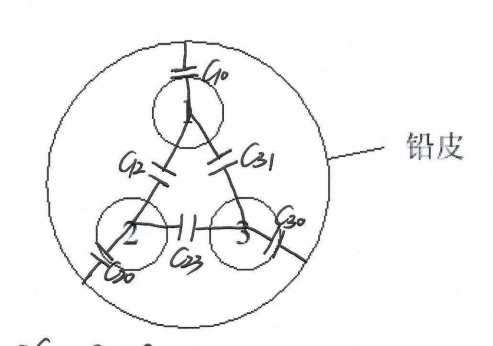
\includegraphics[width=0.6\textwidth]{4.13.png}
\end{center}

\textbf{解答：}

设对称三芯电缆的各部分电容为：
- 导体与铅皮间的电容为 \(C_0\)（每相）
- 导体间的电容为 \(C_1\)（每两相之间）

根据题意，两次测量的电容值可表示为：
1.  三导体相联，与铅皮间的电容：
    \[
    3C_0 = 0.051\,\mu\text{F}
    \]
2.  两导体与铅皮相联，与另一导体间的电容：
    \[
    C_0 + 2C_1 = 0.037\,\mu\text{F}
    \]

\vspace{0.5em}
(1) 求解各部分电容：
由第一个方程得：
\[
C_0 = \frac{0.051}{3} = 0.017\,\mu\text{F}
\]
代入第二个方程：
\[
0.017 + 2C_1 = 0.037 \implies C_1 = \frac{0.037 - 0.017}{2} = 0.01\,\mu\text{F}
\]
因此，电缆的各部分电容为：\(C_0 = 0.017\,\mu\text{F}\)，\(C_1 = 0.01\,\mu\text{F}\)。

\vspace{0.5em}
(2) 每一相的工作电容：
三相对称工作时，每一相的工作电容（导体对地的等效电容）为：
\[
C_\text{ph} = C_0 + 3C_1 = 0.017 + 3 \times 0.01 = 0.047\,\mu\text{F}
\]

\vspace{0.5em}
(3) 导体1、2间加 \(100\,\text{V}\) 电压时的单位长度电荷量：
此时，两导体间的等效电路为：两导体之间通过工作电容 \(C_\text{ph}\) 形成对称结构，可等效为两个串联的 \(C_\text{ph}\) 电容接在 \(100\,\text{V}\) 电压上。
根据电容电荷公式，导体的电荷量为：
\[
Q = \frac{1}{2} C_\text{ph} U
\]
代入数值：
\[
Q = \frac{1}{2} \times 0.047\,\mu\text{F} \times 100\,\text{V} = 2.35\,\mu\text{C}
\]
因此，导体每单位长度的电荷量为 \(2.35\,\mu\text{C}\)。

\vspace{1em}

% 第14题
\item 图(a)所示为镜像法分析静电场分布特性问题。两个点电荷分别位于两种介质中，两种介质的分界面为无限大平面，介电常数分别为 \(\varepsilon_1\) 和 \(\varepsilon_2\)，点电荷 \(q_1\) 与 \(q_2\) 相对于界面为镜像位置，相距为 \(2h\)。用叠加定理分析介质1中的电位 \(\varphi_1\)。当点电荷 \(q_1\) 单独作用时，可按图(b)计算，在图(b)的括号中填入相应的介电常数，此时 \(q_1' = \frac{\varepsilon_1 - \varepsilon_2}{\varepsilon_1 + \varepsilon_2} q_1\)；当点电荷 \(q_2\) 单独作用时，可按图(c)计算，在图(c)的括号中填入相应的介电常数，此时 \(q_2'' = \frac{2\varepsilon_1}{\varepsilon_1 + \varepsilon_2} q_2\)。

\begin{center}
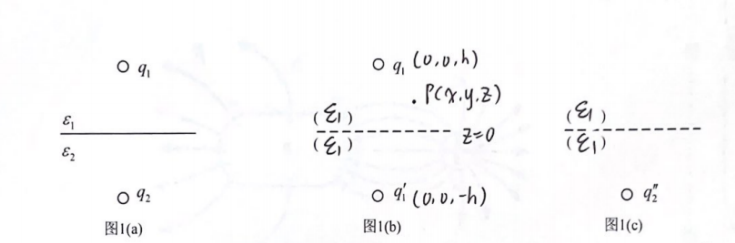
\includegraphics[width=0.8\textwidth]{4.14.png}
\end{center}

\textbf{解答：}

\vspace{0.5em}
(1) 图(b)中，点电荷 \(q_1\) 位于介质1中，为了计算介质1中的电位，需要在介质2中引入镜像电荷 \(q_1'\)。此时，整个空间视为充满介电常数为 \(\varepsilon_1\) 的介质。因此，图(b)的两个括号中均应填入 \(\boxed{\varepsilon_1}\)。
镜像电荷 \(q_1'\) 的大小为：
\[
q_1' = \frac{\varepsilon_1 - \varepsilon_2}{\varepsilon_1 + \varepsilon_2} q_1
\]

\vspace{0.5em}
(2) 图(c)中，点电荷 \(q_2\) 位于介质2中，为了计算介质1中的电位，需要将其等效为位于介质1中的点电荷 \(q_2''\)。此时，整个空间视为充满介电常数为 \(\varepsilon_1\) 的介质。因此，图(c)的括号中应填入 \(\boxed{\varepsilon_1}\)。
等效点电荷 \(q_2''\) 的大小为：
\[
q_2'' = \frac{2\varepsilon_1}{\varepsilon_1 + \varepsilon_2} q_2
\]

\vspace{0.5em}
(3) 介质1中的电位 \(\varphi_1\) 由 \(q_1\) 和 \(q_2\) 共同作用叠加而成：
\[
\varphi_1 = \frac{1}{4\pi\varepsilon_1} \left( \frac{q_1}{r_1} + \frac{q_1'}{r_1'} + \frac{q_2''}{r_2} \right)
\]
其中 \(r_1\) 为场点到 \(q_1\) 的距离，\(r_1'\) 为场点到镜像电荷 \(q_1'\) 的距离，\(r_2\) 为场点到 \(q_2\) 的距离。

\vspace{1em}

% 第15题
\item 试求无限长同轴电容器的单位长度电容。

\begin{center}
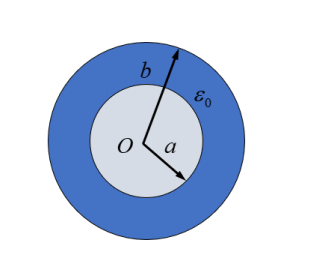
\includegraphics[width=0.4\textwidth]{4.15.png}
\end{center}

\textbf{解答：}

假设内导体的线电荷为 \(\tau\)，根据电荷分布的轴对称性，利用高斯定理求解内外导体间的电场强度。

取半径为 \(r\)、长度为 \(h\) 的同轴圆柱面为高斯面，由高斯定理：
\[
Q = \oint_S \vec{D} \cdot d\vec{S}
\]

高斯面内包围的电荷为 \(Q = \tau h\)，电位移矢量 \(\vec{D} = \varepsilon_0 \vec{E}\)，电场仅沿径向 \(\vec{e}_r\) 方向，因此：
\[
\tau h = \varepsilon_0 E \cdot 2\pi r h
\]

解得电场强度：
\[
\vec{E} = \frac{\tau}{2\pi\varepsilon_0 r} \vec{e}_r
\]

同轴柱面之间的电压为：
\[
U = \int_{a}^{b} \vec{E} \cdot d\vec{r} = \int_{a}^{b} \frac{\tau}{2\pi\varepsilon_0 r} dr = \frac{\tau}{2\pi\varepsilon_0} \ln \frac{b}{a}
\]

根据电容定义，单位长度的电容为：
\[
C = \frac{\tau}{U} = \frac{2\pi\varepsilon_0}{\ln(b/a)}
\]

\end{enumerate}     % 你原来的静电场章节
\section{恒定电场习题解答}

\begin{enumerate}

\item （1分）在导电媒质中，电荷的体密度为
\[
\rho = \nabla\left(\frac{\varepsilon}{\gamma}\right)\cdot\vec{J}
\]
当导电媒质为均匀媒质时，$\varepsilon$ 和 $\gamma$ 都不随空间位置变化，因此电荷密度为零。另一方面，由定义可知，体电流密度为电荷体密度乘以电荷的运动速度。试解释均匀导电媒质中体电流密度不为零而体电荷密度为零这一“矛盾”。

解答：
均匀导电媒质中，$\varepsilon$、$\gamma$ 为常数，故
\[
\nabla\left(\frac{\varepsilon}{\gamma}\right)=0\implies\rho=0
\]
这表示净体电荷密度为零，并不代表不存在电荷。导体中存在大量可自由移动的正负电荷（如金属中的自由电子和晶格正离子），它们的体密度大小相等、符号相反，叠加后净密度为零。

当外加电场时，正负电荷在电场力作用下定向运动：
正电荷沿电场方向运动，负电荷逆电场方向运动，两者的运动方向相反，但电流方向一致，因此会形成不为零的体电流密度 $\vec{J}$。
整个过程中，正负电荷的体密度始终保持大小相等、符号相反，净体电荷密度仍为零。

因此，“净体电荷密度为零”与“体电流密度不为零”并不矛盾。

\item （4分）球形电容器内半径 $R_1=5\,\text{cm}$，外半径 $R_2=10\,\text{cm}$，内外导体间的非理想电介质的电导率 $\gamma=10^{-9}\,\text{S/m}$，若内外导体间电压 $U_0=1000\,\text{V}$，求内外导体间的 $\varphi$、$\vec{E}$、$\vec{J}$ 和绝缘电阻 $R$。

解答：
设内导体流出的总电流为 $I$，由对称性，电流密度为径向分布：
\[
\vec{J} = \frac{I}{4\pi r^2}\vec{e}_r,\quad R_1<r<R_2
\]
由欧姆定律 $\vec{J}=\gamma\vec{E}$，得电场：
\[
\vec{E} = \frac{I}{4\pi\gamma r^2}\vec{e}_r
\]
内外导体间电压：
\[
U_0 = \int_{R_1}^{R_2} \vec{E}\cdot d\vec{r} = \frac{I}{4\pi\gamma}\left(\frac{1}{R_1}-\frac{1}{R_2}\right)
\]
解得总电流：
\[
I = \frac{4\pi\gamma U_0 R_1 R_2}{R_2-R_1}
\]

(1) 电场强度：
\[
\vec{E} = \frac{U_0 R_1 R_2}{(R_2-R_1)r^2}\vec{e}_r
\]

(2) 电流密度：
\[
\vec{J} = \gamma\vec{E} = \frac{\gamma U_0 R_1 R_2}{(R_2-R_1)r^2}\vec{e}_r
\]

(3) 电位（以外导体为参考点，$\varphi(R_2)=0$）：
\[
\varphi(r) = \int_r^{R_2} \vec{E}\cdot d\vec{r} = \frac{U_0 R_1 R_2}{R_2-R_1}\left(\frac{1}{r}-\frac{1}{R_2}\right)
\]

(4) 绝缘电阻：
\[
R = \frac{U_0}{I} = \frac{1}{4\pi\gamma}\left(\frac{1}{R_1}-\frac{1}{R_2}\right)
\]
代入数值：
\[
R = \frac{1}{4\pi\times10^{-9}}\left(\frac{1}{0.05}-\frac{1}{0.1}\right) \approx 1.59\times10^9\,\Omega
\]

\item （5分）同轴电缆内导体半径为 $R_1$，外导体半径为 $R_3$，内外导体之间有两层媒质。内层从 $R_1$ 到 $R_2$，媒质的参数为 $\varepsilon_{r1}$ 和 $\gamma_1$；外层从 $R_2$ 到 $R_3$，媒质的参数为 $\varepsilon_{r2}$ 和 $\gamma_2$。求：
\begin{enumerate}
    \item 每层单位长度的电容；
    \item 每层单位长度的电导；
    \item 单位长度的总电容；
    \item 单位长度的总电导；
    \item 当同轴电缆长度为 $L$，内外导体之间的电压为 $U$，忽略边缘效应，利用边界上的衔接条件分别求界面 $R_1$、$R_2$ 和 $R_3$ 上的电荷面密度。
\end{enumerate}

解答：
设单位长度电荷为 $\tau$，单位长度漏电流为 $I_0$。

(1) 单位长度电容：
内层（$R_1\sim R_2$）：
\[
C_{01} = \frac{2\pi\varepsilon_1}{\ln(R_2/R_1)},\quad \varepsilon_1=\varepsilon_0\varepsilon_{r1}
\]
外层（$R_2\sim R_3$）：
\[
C_{02} = \frac{2\pi\varepsilon_2}{\ln(R_3/R_2)},\quad \varepsilon_2=\varepsilon_0\varepsilon_{r2}
\]

(2) 单位长度电导：
内层（$R_1\sim R_2$）：
\[
G_{01} = \frac{2\pi\gamma_1}{\ln(R_2/R_1)}
\]
外层（$R_2\sim R_3$）：
\[
G_{02} = \frac{2\pi\gamma_2}{\ln(R_3/R_2)}
\]

(3) 单位长度总电容（两层串联）：
\[
\frac{1}{C_0} = \frac{1}{C_{01}}+\frac{1}{C_{02}} \implies C_0 = \frac{C_{01}C_{02}}{C_{01}+C_{02}}
\]

(4) 单位长度总电导（两层串联）：
\[
\frac{1}{G_0} = \frac{1}{G_{01}}+\frac{1}{G_{02}} \implies G_0 = \frac{G_{01}G_{02}}{G_{01}+G_{02}}
\]

(5) 界面电荷面密度：
由电流连续性，两层电流密度法向连续：$J_{1n}=J_{2n}$，即
\[
\gamma_1 E_1 = \gamma_2 E_2 = J_0
\]
电压：
\[
U = E_1\ln\frac{R_2}{R_1} + E_2\ln\frac{R_3}{R_2}
\]
解得：
\[
E_1 = \frac{U\gamma_2}{\gamma_2\ln\frac{R_2}{R_1}+\gamma_1\ln\frac{R_3}{R_2}},\quad E_2 = \frac{U\gamma_1}{\gamma_2\ln\frac{R_2}{R_1}+\gamma_1\ln\frac{R_3}{R_2}}
\]
$R_1$ 处：
\[
\sigma_1 = \varepsilon_1 E_1 = \frac{\varepsilon_1 U\gamma_2}{\gamma_2\ln\frac{R_2}{R_1}+\gamma_1\ln\frac{R_3}{R_2}}
\]
$R_2$ 处：
\[
\sigma_2 = \varepsilon_2 E_2 - \varepsilon_1 E_1 = \frac{U(\varepsilon_2\gamma_1-\varepsilon_1\gamma_2)}{\gamma_2\ln\frac{R_2}{R_1}+\gamma_1\ln\frac{R_3}{R_2}}
\]
$R_3$ 处：
\[
\sigma_3 = -\varepsilon_2 E_2 = -\frac{\varepsilon_2 U\gamma_1}{\gamma_2\ln\frac{R_2}{R_1}+\gamma_1\ln\frac{R_3}{R_2}}
\]

\item （1分）假设大地为均匀导电媒质，浅埋于地下的不规则形状接地体电流流入大地。在远离接地体的大地内，电流如何分布？

解答：
在远离接地体的区域，接地体可近似看作点电流源，电流以径向对称的方式向四周扩散。

电流密度分布为：
\[
\vec{J} = \frac{I}{2\pi r^2}\vec{e}_r
\]
对应的电场强度为：
\[
\vec{E} = \frac{\vec{J}}{\gamma} = \frac{I}{2\pi\gamma r^2}\vec{e}_r
\]
电流呈球面辐射状分布，且随着距离 $r$ 的增大，电流密度按 $1/r^2$ 规律衰减。

\item （3分）平行平板电容器，两极板间距为 $d$，极板之间有两种电介质，第一种电介质厚度为 $a$，介电常数为 $\varepsilon_1$，电导率为 $\gamma_1$；第二种电介质厚度为 $d-a$，介电常数为 $\varepsilon_2$，电导率为 $\gamma_2$。若两极板间加电压 $U$，求电介质中的电场强度、漏电流密度和电介质分界面上的自由电荷面密度。

解答：
由电流连续性，两种介质中漏电流密度相等，设为 $J$，则：
\[
E_1 = \frac{J}{\gamma_1},\quad E_2 = \frac{J}{\gamma_2}
\]
电压关系：
\[
U = E_1 a + E_2 (d-a) = J\left(\frac{a}{\gamma_1}+\frac{d-a}{\gamma_2}\right)
\]
解得：
\[
J = \frac{U\gamma_1\gamma_2}{\gamma_2 a + \gamma_1(d-a)}
\]

(1) 电场强度：
\[
E_1 = \frac{U\gamma_2}{\gamma_2 a + \gamma_1(d-a)},\quad E_2 = \frac{U\gamma_1}{\gamma_2 a + \gamma_1(d-a)}
\]

(2) 漏电流密度：
\[
J = \frac{U\gamma_1\gamma_2}{\gamma_2 a + \gamma_1(d-a)}
\]

(3) 分界面自由电荷面密度：
\[
\sigma = \varepsilon_2 E_2 - \varepsilon_1 E_1 = \frac{U(\varepsilon_2\gamma_1-\varepsilon_1\gamma_2)}{\gamma_2 a + \gamma_1(d-a)}
\]

\item （2分）在恒定电场的电源中，总的电场强度闭合线积分为零吗？局外电场强度的闭合线积分为零吗？库仑电场强度的闭合线积分为零吗？在电源之外，上述3个闭合线积分是否为零？

解答：
设电源内的总电场为 $\vec{E}=\vec{E}_c+\vec{E}_e$，其中 $\vec{E}_c$ 为库仑电场，$\vec{E}_e$ 为局外电场。

电源内部：
总电场：$\oint \vec{E}\cdot d\vec{l} = \oint (\vec{E}_c+\vec{E}_e)\cdot d\vec{l} \neq 0$
局外电场：$\oint \vec{E}_e\cdot d\vec{l} \neq 0$
库仑电场：$\oint \vec{E}_c\cdot d\vec{l} = 0$

电源外部：
局外电场 $\vec{E}_e=0$，总电场等于库仑电场，因此：
\[
\oint \vec{E}\cdot d\vec{l} = \oint \vec{E}_c\cdot d\vec{l} = 0
\]
三个积分均为零。

\item （2分）请依据电流密度矢量 $\vec{J}$ 的定义及电流连续性定理，分别给出电路理论中焦耳定律（微分形式）与基尔霍夫电流定律的推导过程。

解答：
焦耳定律（微分形式）推导：
单位体积内的功率损耗（焦耳热）等于电场力对电荷做功的功率。
由欧姆定律 $\vec{J}=\gamma\vec{E}$，单位体积功率：
\[
p = \vec{J}\cdot\vec{E} = \gamma E^2
\]
即焦耳定律的微分形式：$p=\vec{J}\cdot\vec{E}$。

基尔霍夫电流定律（KCL）推导：
电流连续性定理：
\[
\nabla\cdot\vec{J} = -\frac{\partial\rho}{\partial t}
\]
恒定电流下 $\frac{\partial\rho}{\partial t}=0$，故 $\nabla\cdot\vec{J}=0$。
对节点取闭合面，由高斯定理：
\[
\oiint_S \vec{J}\cdot d\vec{S} = 0
\]
即流入节点的电流之和等于流出节点的电流之和，对应KCL：
\[
\sum I_k = 0
\]

\end{enumerate}
% !TeX root = main.tex
\section{恒定磁场}
\begin{enumerate}
    \item 已知无限长直导体圆柱由电导率不同的两层导体构成，内层导体的半径 $R_1=2\,\text{mm}$，电导率 $\gamma_1=10^7\,\text{S/m}$；外层导体的外半径 $R_2=3\,\text{mm}$，电导率 $\gamma_2=4\times10^7\,\text{S/m}$。导体圆柱中沿轴线方向流过的电流为 $I=100\,\text{A}$，求：
    \begin{enumerate}
        \item 两层导体中的电流密度 $\vec{J}_1$ 和 $\vec{J}_2$；
        \item 导体圆柱内、外的磁感应强度。
    \end{enumerate}

    \paragraph{解答：}
    \begin{enumerate}
        \item 由于两层导体串联，电场强度 $E$ 相同，电流密度满足 $J=\gamma E$，故 $J_1=\gamma_1 E$，$J_2=\gamma_2 E$。
        设内层电流为 $I_1$，外层电流为 $I_2$，则 $I=I_1+I_2$。
        \[
        I_1 = J_1 \pi R_1^2 = \gamma_1 E \pi R_1^2, \quad I_2 = J_2 \pi (R_2^2-R_1^2) = \gamma_2 E \pi (R_2^2-R_1^2)
        \]
        代入数据 $R_1=2\times10^{-3}\,\text{m}$，$R_2=3\times10^{-3}\,\text{m}$，解得：
        \[
        E = \frac{I}{\pi\left(\gamma_1 R_1^2 + \gamma_2(R_2^2-R_1^2)\right)}
        \]
        \[
        J_1 = \gamma_1 E = \frac{I \gamma_1}{\pi\left(\gamma_1 R_1^2 + \gamma_2(R_2^2-R_1^2)\right)} = 2.5\times10^6\,\text{A/m}^2
        \]
        \[
        J_2 = \gamma_2 E = \frac{I \gamma_2}{\pi\left(\gamma_1 R_1^2 + \gamma_2(R_2^2-R_1^2)\right)} = 1.0\times10^7\,\text{A/m}^2
        \]
        方向均沿轴线方向。

        \item 由安培环路定理 $\oint \vec{H}\cdot d\vec{l}=I_{\text{enclosed}}$：
        \begin{itemize}
            \item 当 $0<\rho<R_1$：
            \[
            H \cdot 2\pi\rho = J_1 \pi\rho^2 \Rightarrow H = \frac{J_1 \rho}{2}, \quad B = \mu_0 H = \frac{\mu_0 J_1 \rho}{2}
            \]
            \item 当 $R_1<\rho<R_2$：
            \[
            H \cdot 2\pi\rho = I_1 + J_2 \pi(\rho^2-R_1^2) \Rightarrow B = \mu_0 H
            \]
            \item 当 $\rho>R_2$：
            \[
            H \cdot 2\pi\rho = I \Rightarrow B = \frac{\mu_0 I}{2\pi\rho}
            \]
        \end{itemize}
    \end{enumerate}

    \item 有一半径为 $a$ 的长直圆柱形导体，通有电流密度为 $\vec{J}=J_0\frac{\rho}{a}\vec{e}_z$ 的恒定电流（$z$ 轴就是圆柱导体的轴线）。试求导体内、外的磁场强度 $\vec{H}$。

    \paragraph{解答：}
    由安培环路定理，磁场仅沿 $\vec{e}_\theta$ 方向，大小仅与 $\rho$ 有关。
    \begin{itemize}
        \item 当 $0<\rho<a$：
        \[
        I_{\text{enclosed}} = \int_0^\rho \int_0^{2\pi} J_0 \frac{\rho'}{a} \rho' d\rho' d\theta = \frac{2\pi J_0}{3a}\rho^3
        \]
        \[
        H \cdot 2\pi\rho = I_{\text{enclosed}} \Rightarrow H = \frac{J_0 \rho^2}{3a} \Rightarrow \vec{H} = \frac{J_0 \rho^2}{3a}\vec{e}_\theta
        \]
        \item 当 $\rho>a$：
        \[
        I = \int_0^a \int_0^{2\pi} J_0 \frac{\rho'}{a} \rho' d\rho' d\theta = \frac{2\pi J_0 a^2}{3}
        \]
        \[
        H \cdot 2\pi\rho = I \Rightarrow H = \frac{J_0 a^2}{3\rho} \Rightarrow \vec{H} = \frac{J_0 a^2}{3\rho}\vec{e}_\theta
        \]
    \end{itemize}

    \item 一根截面积为 $2\,\text{cm}^2$，长为 $10\,\text{cm}$ 的圆柱状磁媒质被均匀磁化，磁化强度 $\vec{M}=2\vec{e}_x\,\text{(A/m)}$，试计算它的磁矩 $\vec{m}$。

    \paragraph{解答：}
    磁矩与磁化强度的关系为 $\vec{m} = \vec{M} V$，其中 $V$ 为体积。
    \[
    V = S l = 2\times10^{-4}\,\text{m}^2 \times 0.1\,\text{m} = 2\times10^{-5}\,\text{m}^3
    \]
    \[
    \vec{m} = 2\vec{e}_x \times 2\times10^{-5} = 4\times10^{-5}\vec{e}_x\,\text{(A·m}^2\text{)}
    \]

    \item $z=0$ 是两种媒质的分界面，分界面上无自由电流密度分布，在 $z>0$ 时，$\mu_{r1}=1$，$\vec{B}_1=1.5\vec{e}_x+0.8\vec{e}_y+0.6\vec{e}_z\,\text{mT}$；在 $z<0$ 时，$\mu_{r2}=100$，求：
    \begin{enumerate}
        \item 在 $z<0$ 时的磁感应强度 $\vec{B}_2$；
        \item 每个区域的磁化强度和界面磁化面电流密度。
    \end{enumerate}

    \paragraph{解答：}
    设分界面法向为 $\vec{e}_z$，无自由电流时，切向分量 $H_{1t}=H_{2t}$，法向分量 $B_{1n}=B_{2n}$。
    \begin{enumerate}
        \item $B_{2z}=B_{1z}=0.6\,\text{mT}$。
        $H_{1x} = \frac{B_{1x}}{\mu_0\mu_{r1}} = \frac{1.5\times10^{-3}}{\mu_0}$，$H_{1y} = \frac{0.8\times10^{-3}}{\mu_0}$。
        由 $H_{2x}=H_{1x}, H_{2y}=H_{1y}$，得：
        \[
        B_{2x} = \mu_0\mu_{r2}H_{2x} = 100 \times 1.5\times10^{-3} = 150\,\text{mT}
        \]
        \[
        B_{2y} = \mu_0\mu_{r2}H_{2y} = 100 \times 0.8\times10^{-3} = 80\,\text{mT}
        \]
        故 $\vec{B}_2 = 150\vec{e}_x + 80\vec{e}_y + 0.6\vec{e}_z\,\text{mT}$。

        \item 磁化强度 $\vec{M} = \frac{\vec{B}}{\mu_0} - \vec{H}$：
        \[
        \vec{M}_1 = \left(\frac{1.5\vec{e}_x+0.8\vec{e}_y+0.6\vec{e}_z}{\mu_0} - \frac{1.5\vec{e}_x+0.8\vec{e}_y+0.6\vec{e}_z}{\mu_0}\right) = 0
        \]
        \[
        \vec{M}_2 = \left(\frac{150\vec{e}_x+80\vec{e}_y+0.6\vec{e}_z}{\mu_0} - \frac{1.5\vec{e}_x+0.8\vec{e}_y+0.6\vec{e}_z}{\mu_0}\right) = \frac{148.5\vec{e}_x + 79.2\vec{e}_y}{\mu_0}\times10^{-3}\,\text{A/m}
        \]
        界面磁化面电流密度：
        \[
        \vec{J}_{ms} = \vec{e}_z \times (\vec{M}_2 - \vec{M}_1) = \vec{e}_z \times \vec{M}_2 = \frac{1}{\mu_0}(-79.2\vec{e}_x + 148.5\vec{e}_y)\times10^{-3}\,\text{A/m}
        \]
    \end{enumerate}

    \item 证明在平行平面磁场中等 $\vec{A}$ 线就是 $\vec{B}$ 线。

    \paragraph{解答：}
    平行平面磁场中，矢量磁位 $\vec{A}$ 仅有 $z$ 分量，即 $\vec{A}=A_z(x,y)\vec{e}_z$，且 $\vec{B}=\nabla\times\vec{A}$。
    \[
    \vec{B} = \nabla\times(A_z\vec{e}_z) = \frac{\partial A_z}{\partial y}\vec{e}_x - \frac{\partial A_z}{\partial x}\vec{e}_y
    \]
    等 $\vec{A}$ 线满足 $A_z(x,y)=\text{常数}$，其切线方向为 $\left(\frac{\partial A_z}{\partial y}, -\frac{\partial A_z}{\partial x}\right)$，与 $\vec{B}$ 的方向完全一致，故等 $\vec{A}$ 线就是 $\vec{B}$ 线。

    \item 一根极细的圆铁杆和一个很薄的圆铁盘样品放入磁场 $\vec{B}_0$ 中，并使它们的轴与 $\vec{B}_0$ 平行，铁的磁导率为 $\mu$，求两样样品内的 $\vec{B}$，$\vec{H}$。若已知 $\vec{B}_0=1\,\text{T}$，$\mu=5000\mu_0$，求两样样品内的磁化强度 $\vec{M}$。

    \paragraph{解答：}
    \begin{itemize}
        \item 极细圆铁杆：退磁因子 $N\approx0$，内部磁场 $H=H_0$，故：
        \[
        B = \mu H = \mu H_0 = \frac{\mu}{\mu_0}B_0 = 5000\,\text{T}
        \]
        \[
        M = \frac{B}{\mu_0} - H = \left(\frac{5000\mu_0}{\mu_0} - \frac{1}{\mu_0}\right)B_0 = \frac{4999}{\mu_0}\,\text{A/m}
        \]

        \item 很薄圆铁盘：退磁因子 $N\approx1$，内部磁场 $H=H_0 - N M = H_0 - M$，且 $B=\mu(H_0 - M)=\mu_0(H_0 + M)$，解得：
        \[
        M = \frac{\mu-\mu_0}{\mu+\mu_0}H_0 \approx H_0, \quad B=\mu_0(H_0+M) \approx B_0=1\,\text{T}
        \]
        \[
        H = H_0 - M \approx 0, \quad M = \frac{B}{\mu_0} - H \approx \frac{1}{\mu_0}\,\text{A/m}
        \]
    \end{itemize}

    \item 在真空均匀磁场中放入一小块铁磁媒质（相对磁导率远大于 1），试问与周围场域相比，媒质中磁感应强度和磁场强度总体有何变化（大或小）？

    \paragraph{解答：}
    - 磁感应强度 $B$：由于铁磁媒质被强烈磁化，产生附加磁场，故媒质中 $B$ 显著增大。
    - 磁场强度 $H$：在退磁效应影响下，媒质内部 $H$ 比外部真空的 $H_0$ 小（退磁场与外场反向）。

    \item 无限长同轴电缆横截面如图所示，内外导体通过等大反向恒定电流，外导体电流均匀分布，内导体电流密度为
    \[
    \vec{J} = -\frac{I}{\pi\rho_1^2}\vec{e}_z
    \]

    \begin{enumerate}
        \item 计算内导体磁感应强度；
        \item 计算内外导体之间的磁感应强度。
    \end{enumerate}

    \paragraph{解答：}
    由安培环路定理，磁场仅沿 $\vec{e}_\theta$ 方向。
    \begin{enumerate}
        \item 内导体（$0<\rho<\rho_1$）：
        \[
        I_{\text{enclosed}} = \int_0^\rho J \cdot 2\pi\rho' d\rho' = \frac{I\rho^2}{\rho_1^2}
        \]
        \[
        H \cdot 2\pi\rho = I_{\text{enclosed}} \Rightarrow H = \frac{I\rho}{2\pi\rho_1^2}
        \]
        \[
        B = \mu_0 H = \frac{\mu_0 I \rho}{2\pi\rho_1^2}\vec{e}_\theta
        \]

        \item 内外导体之间（$\rho_1<\rho<\rho_2$）：
        包围电流为内导体全部电流 $I$，故：
        \[
        H \cdot 2\pi\rho = I \Rightarrow H = \frac{I}{2\pi\rho}
        \]
        \[
        B = \mu_0 H = \frac{\mu_0 I}{2\pi\rho}\vec{e}_\theta
        \]
    \end{enumerate}

    \item 同轴电缆内导体半径为 $0.5\,\text{m}$，外导体半径为 $1\,\text{m}$，长度为 $2\,\text{m}$。电缆中的电流为 $5\,\text{A}$，绝缘材料的磁导率为 $\mu_0$，计算在半径为 $0.75\,\text{m}$ 处的磁场能量密度。

    \paragraph{解答：}
    $0.75\,\text{m}$ 位于内外导体之间，磁场强度为：
    \[
    H = \frac{I}{2\pi\rho} = \frac{5}{2\pi \times 0.75} = \frac{10}{3\pi}\,\text{A/m}
    \]
    磁场能量密度：
    \[
    w_m = \frac{1}{2}\mu_0 H^2 = \frac{1}{2}\mu_0 \left(\frac{10}{3\pi}\right)^2 = \frac{50\mu_0}{9\pi^2}\,\text{J/m}^3
    \]
    代入 $\mu_0=4\pi\times10^{-7}\,\text{H/m}$，得：
    \[
    w_m = \frac{50 \times 4\pi\times10^{-7}}{9\pi^2} = \frac{200\times10^{-7}}{9\pi} \approx 7.07\times10^{-7}\,\text{J/m}^3
    \]
\end{enumerate}
\section{时变电磁场大作业解答}
\begin{enumerate}[label=\arabic*.]

\item 同轴电缆中的 TEM 波
已知内导体半径 \(a=1\,\text{mm}\)，外导体半径 \(b=4\,\text{mm}\)，介质聚乙烯 \(\varepsilon_r=2.25,\ \mu_r=1,\ \gamma=0\)，电场
\[
\vec{E} = \frac{100}{\rho}\cos(10^8 t - \beta z)\,\vec{e}_\rho\ \text{V/m}
\]
\begin{enumerate}[label=(\arabic*)]
    \item 判断电场表达式是否具有波动性
    场量含行波因子 \(\cos(\omega t-\beta z)\)，沿 \(+z\) 方向传播，因此**具有波动性**。

    \item 求解相位常数 \(\beta\)
    \[
    \beta = \omega\sqrt{\mu_0\varepsilon_0\varepsilon_r} = \frac{\omega}{c}\sqrt{\varepsilon_r}
    \]
    代入 \(\omega=10^8\,\text{rad/s},\ c=3\times 10^8\,\text{m/s},\sqrt{\varepsilon_r}=1.5\)
    \[
    \beta = \frac{10^8}{3\times 10^8}\times 1.5 = \boldsymbol{0.5\ \text{rad/m}}
    \]

    \item 求解磁场强度 \(\vec{H}\) 表达式
    由 \(\nabla\times\vec{E}=-\mu_0\dfrac{\partial\vec{H}}{\partial t}\)，圆柱坐标旋度展开得
    \[
    \nabla\times\vec{E} = \frac{100\beta}{\rho}\sin(\omega t-\beta z)\,\vec{e}_\phi
    \]
    积分求得磁场分量，介质波阻抗 \(\eta=\dfrac{\eta_0}{\sqrt{\varepsilon_r}}=80\pi\ \Omega\)
    \[
    \vec{H} = \frac{100}{80\pi\rho}\cos\left(10^8 t-0.5 z\right)\,\vec{e}_\phi\ \text{A/m}
    \]

    \item 求解内外导体间平均坡印廷矢量
    \[
    \vec{S}_{\text{av}} = \frac{1}{2}\text{Re}\left(\dot{\vec{E}}\times\dot{\vec{H}}^*\right)
    = \boldsymbol{\frac{125}{2\pi\rho^2}\,\vec{e}_z\ \text{W/m}^2}
    \]

    \item 求解内导体表面线电流密度
    由边界关系 \(\vec{J}_s=\vec{e}_\rho\times\vec{H}\)，代入 \(\rho=a=1\,\text{mm}\)
    \[
    \vec{J}_s = \frac{1250}{\pi}\cos\left(10^8 t-0.5 z\right)\,\vec{e}_z\ \text{A/m}
    \]

    \item 求解 \(0\le z\le 1\,\text{m}\) 区段位移电流
    位移电流密度 \(\vec{J}_d=\varepsilon\dfrac{\partial\vec{E}}{\partial t}\)，对柱面面积分积分化简得
    \[
    I_d \approx -2.5\times 10^{-2}\left[\cos(10^8 t-0.5)-\cos10^8 t\right]\ \text{A}
    \]
\end{enumerate}
\vspace{1em}

\item 平行板电容器中的坡印廷矢量与传输功率
圆形极板面积为 \(S\)，极板间距为 \(d\)，介质参数 \(\varepsilon,\gamma\)。
\begin{enumerate}[label=(\arabic*)]
    \item 直流电压 \(U\) 作用下任一点坡印廷矢量
    极板间均匀电场 \(\vec{E}=\dfrac{U}{d}\vec{e}_z\)，由安培环路定律求得磁场
    \[
    H_\phi = \frac{\gamma U r}{2d}
    \]
    坡印廷矢量
    \[
    \vec{S} = \vec{E}\times\vec{H} = \boldsymbol{-\frac{\gamma U^2 r}{2d^2}\vec{e}_r}
    \]
    能流由侧面径向流入介质内部。

    \item 工频交流电压 \(u=\sqrt{2}U\cos314t\) 下复坡印廷矢量与功率
    角频率 \(\omega=314\,\text{rad/s}\)，写出复场量并推导复坡印廷矢量
    \[
    \dot{\vec{S}} = -\frac{U^2 r}{2d^2}(\gamma-j\omega\varepsilon)\vec{e}_r
    \]
    介质有功损耗功率
    \[
    P = \frac{\gamma S}{d}U^2
    \]
    容性无功功率
    \[
    Q = -\omega C U^2,\quad C=\frac{\varepsilon S}{d}
    \]
\end{enumerate}
\vspace{1em}

\item 无源自由空间场与麦克斯韦方程组验证
\begin{enumerate}[label=(\arabic*)]
    \item 证明仅随时间变化的场不满足麦克斯韦方程组
    以 \(\vec{B}=B_m\sin\omega t\,\vec{e}_z\) 为例，该场无空间分布，旋度 \(\nabla\times\vec{E}=0\)，
    但法拉第电磁感应定律要求旋度等于磁场时变率，二者相互矛盾，故无法满足方程组。

    \item 证明时空联合行波场满足麦克斯韦方程组
    将场改写为 \(\vec{B}=B_m\sin\left[\omega\left(t-\dfrac{y}{c}\right)\right]\vec{e}_z\)，匹配电场与磁场振幅关系 \(E_m=cB_m\)，
    可同时满足法拉第定律与全电流安培定律，符合麦克斯韦方程组约束。

    \item 总结结论与适用条件
    单一时间变化场不属于电磁波解，无法满足时变场基本方程；
    只有形如 \(\cos(\omega t-\beta \boldsymbol{r})\)、兼具时空变化规律的行波场，且满足波速关系 \(\beta=\omega/c\)，才可作为麦克斯韦方程组有效解。
\end{enumerate}
\vspace{1em}

\item 时变电磁场下导线电阻与电感特性分析
恒定场中导线电阻、电感仅由结构尺寸与介质参数决定，与激励无关，该结论**不适用于时变电磁场**。
\textbf{解答：}
\begin{enumerate}
    \item 集肤效应：交变电流集中于导体表层，有效导通截面积减小，交流电阻随工作频率升高显著增大；
    \item 邻近效应：多根载流导线交变磁场相互耦合畸变电流分布，进一步改变等效电路参数；
    \item 频率相关电感：高频下导体内部磁通大幅减少，内电感数值随频率上升持续降低。
\end{enumerate}
综上，时变场中导线等效电阻、等效电感均与工作频率强相关，不再为固定常数。

\end{enumerate}
\section{准静态电磁场习题解答}

\begin{enumerate}[label=\arabic*.]

\item 已知同轴圆柱电容器内半径 \(r_1=1\,\text{cm}\)，外半径 \(r_2=4\,\text{cm}\)，长度 \(l=0.5\,\text{m}\)，介质介电常数 \(\varepsilon=4\varepsilon_0\)，电压 \(u=6000\sqrt{2}\sin100\pi t\,\text{V}\)。求位移电流密度。

\textbf{解答：}
同轴圆柱电容：
\[
C = \frac{2\pi \varepsilon l}{\ln(r_2/r_1)} = \frac{2\pi \cdot 4\varepsilon_0 \cdot 0.5}{\ln 4} = \frac{4\pi \varepsilon_0}{\ln 4}
\]
电场强度（\(r_1<r<r_2\)）：
\[
E(r,t) = \frac{u(t)}{r\ln(r_2/r_1)} = \frac{6000\sqrt{2}\sin100\pi t}{r\ln 4}
\]
位移电流密度：
\[
J_d = \frac{\partial D}{\partial t} = \varepsilon \frac{\partial E}{\partial t}
\]
代入 \(\varepsilon=4\varepsilon_0\)：
\[
J_d(r,t) = 4\varepsilon_0 \cdot \frac{6000\sqrt{2}\cdot 100\pi \cos100\pi t}{r\ln 4}
= \frac{2.4\times 10^6 \sqrt{2}\pi \varepsilon_0}{r\ln 4} \cos100\pi t \quad (\text{A/m}^2)
\]
方向沿径向。

\vspace{1em}

\item 已知球形电容器内半径 \(a\)，外半径 \(b\)，介质介电常数 \(\varepsilon\)，电导率 \(\gamma\)，电压 \(u=U_m\sin\omega t\)。求全电流。

\textbf{解答：}
电场强度（\(a<r<b\)）：
\[
E(r,t) = \frac{u(t)}{r^2\left(\frac{1}{a}-\frac{1}{b}\right)} = \frac{U_m\sin\omega t}{r^2\left(\frac{1}{a}-\frac{1}{b}\right)}
\]
传导电流密度：
\[
J_c = \gamma E = \frac{\gamma U_m\sin\omega t}{r^2\left(\frac{1}{a}-\frac{1}{b}\right)}
\]
位移电流密度：
\[
J_d = \frac{\partial D}{\partial t} = \varepsilon \frac{\partial E}{\partial t} = \frac{\varepsilon \omega U_m\cos\omega t}{r^2\left(\frac{1}{a}-\frac{1}{b}\right)}
\]
全电流（积分 \(J_c+J_d\) 在任意半径 \(r\) 的球面上）：
\[
I = \oint (J_c+J_d)\cdot dS = 4\pi r^2 (J_c+J_d)
= \frac{4\pi U_m}{\frac{1}{a}-\frac{1}{b}} (\gamma \sin\omega t + \varepsilon \omega \cos\omega t)
\]

\vspace{1em}

\item 已知
\[
\vec{E} = 30\pi\cos\left(\omega t-\frac{4}{3}y\right)\vec{e}_z \,\text{V/m}, \quad
\vec{H} = 10\cos\left(\omega t-\frac{4}{3}y\right)\vec{e}_x \,\text{A/m}, \quad \mu_r=1
\]
求 \(\omega\) 和 \(\varepsilon_r\)。

\textbf{解答：}
由法拉第定律 \(\nabla\times\vec{E}=-\mu_0\frac{\partial \vec{H}}{\partial t}\)：
\[
\nabla\times\vec{E} = -\frac{\partial E_z}{\partial y}\vec{e}_x = 40\pi\sin\left(\omega t-\frac{4}{3}y\right)\vec{e}_x
\]
\[
-\mu_0\frac{\partial \vec{H}}{\partial t} = 10\mu_0\omega\sin\left(\omega t-\frac{4}{3}y\right)\vec{e}_x
\]
比较得：
\[
40\pi = 10\mu_0\omega \implies \omega = \frac{4\pi}{\mu_0} = 10^7\,\text{rad/s}
\]

由安培环路定律 \(\nabla\times\vec{H}=\varepsilon_0\varepsilon_r\frac{\partial \vec{E}}{\partial t}\)：
\[
\nabla\times\vec{H} = -\frac{\partial H_x}{\partial y}\vec{e}_z = \frac{40}{3}\sin\left(\omega t-\frac{4}{3}y\right)\vec{e}_z
\]
\[
\varepsilon_0\varepsilon_r\frac{\partial \vec{E}}{\partial t} = -30\pi\omega\varepsilon_0\varepsilon_r\sin\left(\omega t-\frac{4}{3}y\right)\vec{e}_z
\]
比较得：
\[
\frac{40}{3} = 30\pi\omega\varepsilon_0\varepsilon_r
\]
代入 \(\omega=10^7\)，\(\varepsilon_0=8.854\times 10^{-12}\)：
\[
\varepsilon_r = \frac{40}{3\cdot 30\pi \cdot 10^7 \cdot 8.854\times 10^{-12}} \approx 16
\]

\vspace{1em}

\item 已知媒质1（空气，\(\varepsilon_{r1}=1\)），媒质2（干土，\(\varepsilon_{r2}=3\)，\(\gamma_2=10^{-5}\,\text{S/m}\)），
\[
E_1=100\sin(1000t+30^\circ)\,\text{V/m}, \quad \theta_1=45^\circ
\]
求 \(E_2\) 及折射角 \(\theta_2\)。

\textbf{解答：}
角频率 \(\omega=1000\,\text{rad/s}\)，媒质2的损耗正切：
\[
\tan\delta = \frac{\gamma_2}{\omega\varepsilon_0\varepsilon_{r2}} \approx 0.377
\]
属于低损耗介质，近似用无耗边界条件：
切向分量连续 \(E_{1t}=E_{2t}\)，法向分量 \(\varepsilon_1 E_{1n} = \varepsilon_2 E_{2n}\)。

分解 \(E_1\)：
\[
E_{1t} = E_{1n} = 50\sqrt{2}\sin(1000t+30^\circ)
\]
则
\[
E_{2t} = 50\sqrt{2}\sin(1000t+30^\circ),\quad
E_{2n} = \frac{50\sqrt{2}}{3}\sin(1000t+30^\circ)
\]
合场强：
\[
E_2 = \frac{100\sqrt{5}}{3}\sin(1000t+30^\circ)\,\text{V/m}
\]
折射角：
\[
\tan\theta_2 = \frac{E_{2t}}{E_{2n}} = 3 \implies \theta_2 = \arctan 3 \approx 71.6^\circ
\]

\vspace{1em}

\item 已知 \(z=0\) 为空气-理想导体分界面，磁场
\[
\vec{H}(x,y,0,t) = H_0\sin\beta x\cos(\omega t-\beta y)\vec{e}_x
\]
求表面电流密度与切向电场。

\textbf{解答：}
理想导体表面电流密度：
\[
\vec{J}_s = \vec{n}\times\vec{H}
\]
法向 \(\vec{n}=\vec{e}_z\)，故：
\[
\vec{J}_s = H_0\sin\beta x\cos(\omega t-\beta y)\vec{e}_y
\]

理想导体边界切向电场为零：
\[
\vec{E}_t = 0
\]

\vspace{1em}

\item 已知
\[
\vec{E} = 2000\sqrt{2}\sin(\omega t-\beta z)\vec{e}_x\,\text{V/m}, \quad
\vec{H} = 5.3\sqrt{2}\sin(\omega t-\beta z)\vec{e}_y\,\text{A/m}
\]
\(f=20\,\text{MHz}\)，\(\beta=0.42\,\text{rad/m}\)。求瞬时坡印亭矢量、平均坡印亭矢量、净瞬时功率。

\textbf{解答：}
(1) 瞬时坡印亭矢量：
\[
\vec{S}(t) = \vec{E}\times\vec{H}
= 21200\sin^2(\omega t-\beta z)\vec{e}_z \,\text{W/m}^2
\]

(2) 平均坡印亭矢量：
\[
\vec{S}_{av} = \frac{1}{2}\text{Re}\left(\dot{\vec{E}}\times\dot{\vec{H}}^*\right)
= 10600\,\vec{e}_z \,\text{W/m}^2
\]

(3) 平行六面体净瞬时功率（\(A=0.5\,\text{m}^2\)）：
\[
P(t) = 10600\left[\sin^2\omega t - \sin^2(\omega t-0.84)\right]\,\text{W}
\]

\vspace{1em}

\item 圆形平行板电容器（非理想介质），半径 \(a\)，间距 \(d\)，电导率 \(\gamma\)，电压 \(U_0\)。分析能量守恒、电磁场、能流、储能与损耗。

\textbf{解答：}
坡印亭定理：
\[
-\oint_S \vec{S}\cdot d\vec{S} = \frac{d}{dt}\int_V w_e dV + \int_V \gamma E^2 dV
\]

极板间电场：
\[
\vec{E} = \frac{U_0}{d}\vec{e}_z
\]
传导电流密度：
\[
\vec{J} = \frac{\gamma U_0}{d}\vec{e}_z
\]

由安培环路定律得磁场：
\[
\vec{H} = \frac{\gamma U_0 r}{2d}\vec{e}_\phi
\]

坡印亭矢量：
\[
\vec{S} = \vec{E}\times\vec{H}
= -\frac{\gamma U_0^2 r}{2d^2}\vec{e}_r
\]
能流从侧面径向流入介质。

电场能量：
\[
W_e = \frac{\varepsilon \pi a^2}{2d}U_0^2
\]

损耗功率：
\[
P_L = \frac{\gamma \pi a^2}{d}U_0^2
\]
符合坡印亭能量守恒定理。

\end{enumerate}

\end{document}